\documentclass[conference]{IEEEtran}
\usepackage[T1]{fontenc}
\usepackage{cite}
\usepackage{amsmath,amssymb}
\usepackage{graphicx}
\usepackage{booktabs,array}
\usepackage{balance}
\usepackage{tikz}
\usetikzlibrary{arrows.meta,positioning,calc,fit}
\usepackage[hidelinks]{hyperref}
\hypersetup{
  pdftitle={Wearable Gesture Controller: An IMU-Based Edge Device for Gesture-Driven Smart Home Control},
  pdfauthor={Arya Choudhary, Sanika Singh, Vishad Sharma},
  pdfsubject={ICT 3132 Embedded Systems: theoretical mini-project report},
  pdfkeywords={IMU, gesture recognition, accessibility, embedded systems, LSTM, GRU, quantization}}

\begin{document}
\title{Wearable Gesture Controller: An IMU-Based Edge Device for Gesture-Driven Smart Home Control}
\author{\IEEEauthorblockN{Arya Choudhary, Sanika Singh, and Vishad Sharma}
\IEEEauthorblockA{School of Computer Engineering, Manipal Institute of Technology, Manipal, India\\
ICT 3132 Embedded Systems, V Semester B.Tech. (IT)\\
Registration numbers: 240911438, 240911664, and 240911680, respectively}}
\maketitle

\begin{abstract}
Conventional smart-home interfaces may be difficult to use when speech, dexterity, or reach is limited. A wrist-worn inertial measurement unit (IMU) offers a potential alternative by translating intentional wrist movements into appliance-control commands. This report develops a theoretical, platform-independent architecture for such a controller, with local gesture recognition and an optional wireless receiver. The proposed pipeline covers six-axis acquisition, preprocessing, sliding-window segmentation, temporal classification, rejection of uncertain predictions, and command mapping. A baseline long short-term memory (LSTM) network is compared analytically with a compact gated recurrent unit (GRU) network; optional 8-bit post-training quantization is considered subject to runtime compatibility. The design also specifies a future evaluation protocol for classification quality, false activations, latency, memory, and energy. No hardware has been selected or assembled, no dataset has been collected, and no model has been trained or benchmarked. Numerical examples are explicitly analytical illustrations rather than experimental results. The contribution is a technically grounded design and evaluation plan for an accessible embedded interface, with clear limits on what can be concluded without implementation.
\end{abstract}

\begin{IEEEkeywords}
embedded systems, inertial measurement unit, gesture recognition, accessibility, edge inference, GRU, quantization
\end{IEEEkeywords}

\section{Introduction}
Smart-home systems commonly expose touchscreens, handheld remotes, switches, and voice assistants. These interfaces assume particular combinations of reach, speech, and fine motor control. A person with restricted dexterity may find a small button difficult to press, while speech impairment or a noisy room can limit voice interaction. An additional interaction channel could improve access for users who retain some comfortable, repeatable wrist movement. It would complement existing interfaces rather than serve every disability or replace an accessible fallback.

An IMU measures acceleration and angular velocity without observing the surrounding room. Temporal patterns in these signals can represent movements such as a swipe, flick, or wave. Compared with a camera-based interface, a wrist sensor avoids dependence on lighting and line of sight, but introduces sensitivity to sensor placement, incidental movement, and individual motor ability. Gesture recognition must therefore distinguish an intentional command from ordinary activity; classifying isolated gestures alone is insufficient.

The supplied project synopsis motivates a wearable that performs inference locally and communicates a recognized command to a receiver. Local processing can avoid sending raw motion traces to a remote service and can support an internet-independent control path. It does not guarantee security, low latency, or low energy by itself: those properties also depend on firmware, scheduling, communication, and the target device.

This mini-project is deliberately \emph{theoretical}. It adapts the synopsis into a system specification, a focused model comparison, and a reproducible evaluation plan. Data collection, model training, hardware construction, and appliance integration are possible future activities, not requirements or completed deliverables of this report. This distinction applies to all diagrams, tables, and examples below.

\section{Problem Definition and Scope}
\subsection{Problem Statement}
The design problem is to map a short six-axis wrist-motion sequence to a small command vocabulary while respecting the resource constraints of a possible low-power microcontroller. The system must also provide a no-command outcome when motion is incidental or recognition is uncertain. A useful design must account for classification errors, delay, and repeated activations, rather than treating prediction accuracy as its only objective.

\subsection{Objectives and Contributions}
The report has four objectives: define a coherent sensor-to-command architecture; specify a consistent preprocessing and classification pipeline; compare one LSTM baseline with one compact GRU alternative; and describe how recognition quality and embedded feasibility could be evaluated. Its contributions are the proposed architecture, explicit analytical resource estimates, and an evaluation protocol that separates model behaviour from end-to-end system behaviour. It does not claim a new learning algorithm or demonstrated assistive benefit.

\subsection{Scope and Design Assumptions}
The illustrative vocabulary contains four intentional gestures---swipe, flick, wave, and hold---plus a background/no-command class. These are design choices, not an established dataset taxonomy. A hold would require an explicit interaction context and temporal rule because stillness alone is common during normal activity. Gestures and thresholds would need adjustment to a user's range of movement in any future implementation.

The architectural output is a symbolic message, such as \texttt{LIGHT\_ON}. A future receiver could log the message in a software simulation or forward it to a physical actuator. No simulator or receiver has been implemented here. Light control provides a low-consequence running example; door locks and other sensitive actions would require additional confirmation and application-specific safeguards.

\section{Related Work}
Hochreiter and Schmidhuber introduced LSTM to address learning difficulties associated with long temporal dependencies \cite{hochreiter1997}. Its memory cell makes it a useful reference architecture for sequential signals, although the original work does not establish performance on the present gesture vocabulary. Cho \emph{et al.} introduced a gated recurrent encoder--decoder formulation that includes the GRU \cite{cho2014}. A GRU combines gating and recurrent state with fewer gate computations than an LSTM of equal hidden width, motivating its consideration for a constrained device. Neither paper establishes that a GRU will match LSTM accuracy for this application.

Ord\'{o}\~{n}ez and Roggen investigated convolutional and LSTM recurrent networks for multimodal wearable activity recognition \cite{ordonez2016}. Their work supports learning temporal representations from wearable signals, but its activity-recognition setting and richer architecture differ from a small wrist-command interface. Its results cannot be transferred directly to the proposed task or treated as a benchmark for this report.

Jacob \emph{et al.} describe quantization methods for efficient integer-arithmetic inference \cite{jacob2018}. Their work provides a foundation for discussing reduced-precision representations. However, support for quantized recurrent operators, nonlinearities, and state tensors must be verified separately in a chosen embedded runtime. Banbury \emph{et al.} present MLPerf Tiny, which emphasizes evaluating embedded inference through quality, latency, and energy under defined conditions \cite{banbury2021}. This report adopts that multidimensional evaluation principle without claiming to execute, reproduce, or comply with the MLPerf Tiny benchmark suite.

Together, these studies justify a focused investigation of temporal recognition and resource-aware inference. The present report connects those ideas to an accessibility-motivated command interface, with an explicit background class, decision logic, and a platform-independent deployment contract.

\section{Proposed System Architecture}
Fig.~\ref{fig:architecture} describes the proposed logical flow. An IMU supplies three accelerometer and three gyroscope channels. Acquisition associates samples with timestamps and buffers them. Preprocessing conditions the signals, and a classifier produces probabilities for the five illustrative classes. Decision logic suppresses uncertain or repeated predictions before a command mapper creates an output message. A receiver or software-only output stage is the conceptual endpoint; appliance actuation is an optional future extension.

\begin{figure*}[t]
\centering
% Editable vector diagram. All components are proposed, not implemented.
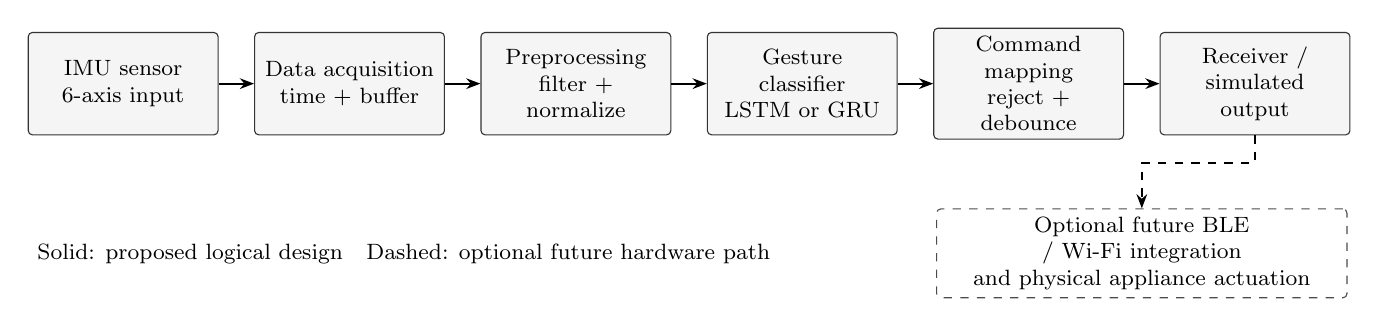
\begin{tikzpicture}[
  font=\footnotesize,
  block/.style={draw=black!80,fill=black!4,rounded corners=1.5pt,
    minimum height=13mm,text width=22mm,align=center,inner sep=3pt},
  optional/.style={draw=black!70,dashed,fill=white,rounded corners=1.5pt,
    minimum height=11mm,text width=50mm,align=center,inner sep=3pt},
  flow/.style={-{Stealth[length=1.8mm]},line width=0.65pt}]
\node[block] (imu) {IMU sensor\\6-axis input};
\node[block,right=4.5mm of imu] (acq) {Data acquisition\\time + buffer};
\node[block,right=4.5mm of acq] (pre) {Preprocessing\\filter + normalize};
\node[block,right=4.5mm of pre] (cls) {Gesture classifier\\LSTM or GRU};
\node[block,right=4.5mm of cls] (map) {Command mapping\\reject + debounce};
\node[block,right=4.5mm of map] (out) {Receiver /\\simulated output};
\foreach \a/\b in {imu/acq,acq/pre,pre/cls,cls/map,map/out}
  \draw[flow] (\a) -- (\b);
\node[optional,below=9mm of $(map.south)!0.5!(out.south)$] (physical)
 {Optional future BLE / Wi-Fi integration\\and physical appliance actuation};
\draw[flow,dashed] (out.south) -- ++(0,-3.5mm) -| (physical.north);
\node[anchor=west,font=\footnotesize,align=left] at ($(imu.south west)+(0,-15mm)$)
 {Solid: proposed logical design\quad Dashed: optional future hardware path};
\end{tikzpicture}

\caption{Proposed sensor-to-command architecture. Solid blocks specify the logical design only; none has been implemented or tested. A receiver could be represented in a future software simulation. Dashed components denote optional physical integration outside the present report's scope.}
\label{fig:architecture}
\end{figure*}

The interface between classification and control is intentionally narrow: a class label, confidence, timestamp, and sequence number. A candidate command would be accepted only when its confidence exceeds a validation-selected threshold and its persistence satisfies a temporal rule. A cooldown or release condition would prevent overlapping windows from issuing the same command repeatedly. Background predictions and stale samples would yield no command. Confidence is not a guarantee of correctness, so rejection behaviour must be evaluated alongside recognition.

For future wireless operation, a message could include a command identifier and acknowledgement request. Sequence checks and timeouts would help avoid duplicate or stale actions, but are not substitutes for authentication. Bluetooth Low Energy (BLE) and local Wi-Fi are alternative transport options; neither is mandatory. Internet independence would require the entire receiver and control path to operate locally. Raw motion data would not need to leave the wearable, although local storage and wireless commands would still need appropriate privacy and access controls.

\section{IMU and Recognition Pipeline}
\subsection{Acquisition and Windowing}
At time index $t$, the input vector is
\begin{equation}
\mathbf{x}_t=[a_x,a_y,a_z,\omega_x,\omega_y,\omega_z]^\mathsf{T},
\end{equation}
where acceleration and angular velocity use fixed, documented units. A nominal sampling frequency of $50$~Hz is an illustrative starting point, not a validated operating requirement. The sensor's range, bandwidth, mounting orientation, timestamp source, and missing-sample policy would be recorded in any future dataset or implementation. Anti-alias filtering must occur before sampling or downsampling; a later digital filter cannot undo aliasing already introduced.

A window of $N=64$ samples with stride $S=16$ would cover $1.28$~s and generate a new decision opportunity every $0.32$~s at the illustrative sampling rate. These values define a trade-off: longer windows may capture complete gestures but can increase response time and include unrelated motion. Neither the window length nor the stride is itself a measured end-to-end latency. Initial window fill, gesture alignment, computation, decision persistence, and communication all contribute to perceived response time.

\subsection{Preprocessing and Feature Representation}
A future pipeline would first check timestamps and flag invalid or incomplete windows. A short causal low-pass filter could suppress high-frequency noise, with coefficients and delay documented. Accelerometer channels contain both gravity and motion; blindly high-pass filtering or subtracting each window's mean could remove information needed for a hold. A fixed calibration and orientation policy should therefore precede any gravity-compensation decision. Accelerometer and gyroscope axes must refer to a consistent mounting convention.

Channel-wise normalization would use training-partition statistics:
\begin{equation}
\widetilde{x}_{t,j}=\frac{x_{t,j}-\mu_j}{\max(\sigma_j,\epsilon)},
\end{equation}
where $j$ indexes the six channels and $\epsilon>0$ prevents division by zero. The same frozen constants would be used during validation, testing, and inference. Computing separate statistics from each test user's full recordings would change the evaluation assumptions and must not occur silently.

The primary feature representation is the ordered $N\times6$ normalized sequence. Both recurrent models learn temporal features from this same input, so handcrafted features are not an additional classifier branch. Window means, standard deviations, root-mean-square values, and acceleration or angular-speed magnitudes could serve as descriptive checks for saturation, activity level, and gesture separability. They would not be appended to one model alone or substituted for the sequence without declaring a changed comparison. This distinction keeps feature extraction explicit while retaining a focused experiment design.

\subsection{Future Data and Split Protocol}
No recordings or dataset statistics are available. If evaluation is later pursued, recordings would need intentional gestures, transitions, and realistic background activities, including movements that resemble commands. Labels should identify gesture intervals, participant, session, and mounting conditions. Consent, data minimization, and comfortable gesture selection would be necessary when involving participants.

Participants or recording sessions must be separated \emph{before} overlapping windows are formed. Otherwise, nearly identical windows can leak across training and test partitions and inflate scores. A held-out-participant protocol would test transfer to new users; a separate within-user protocol could assess personalization. Any augmentation, normalization fitting, class rebalancing, and quantization calibration would use training data only. Validation would select hyperparameters and decision thresholds; the final test partition would remain untouched until evaluation.

\section{Focused Model Comparison}
Fig.~\ref{fig:workflow} summarizes a proposed comparison, not an executed training pipeline. The baseline is a single-layer, unidirectional LSTM with $32$ hidden units and a five-class softmax head. The lightweight alternative is a single-layer GRU with $24$ hidden units and the same output head. Each window starts from a reset recurrent state and uses its final hidden vector for classification. This stateless-window design avoids dependence on earlier windows and keeps the comparison interpretable, at the cost of recomputing overlapping samples.

\begin{figure}[t]
\centering
% Editable vector diagram of a proposed future evaluation, not an executed run.
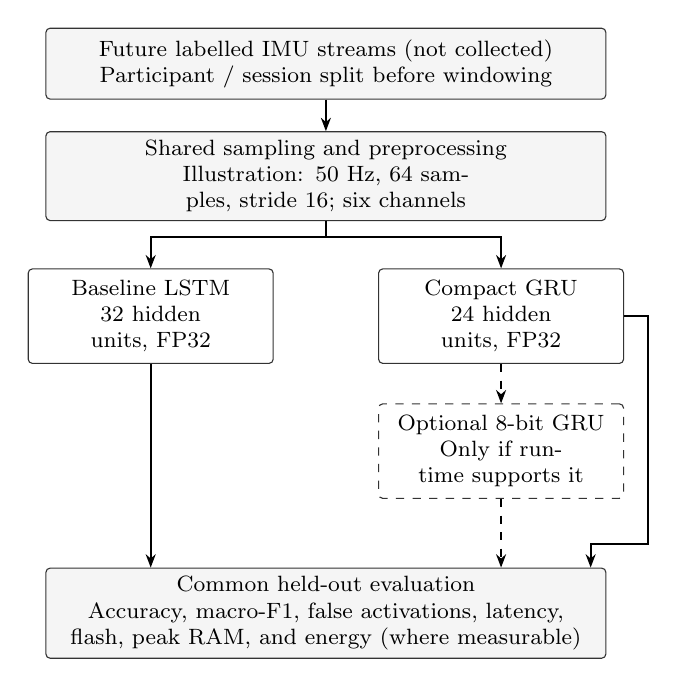
\begin{tikzpicture}[
  font=\footnotesize,
  shared/.style={draw=black!80,fill=black!4,rounded corners=1.5pt,
    text width=69mm,align=center,minimum height=9mm,inner sep=3pt},
  lane/.style={draw=black!80,fill=white,rounded corners=1.5pt,
    text width=29mm,align=center,minimum height=12mm,inner sep=3pt},
  opt/.style={lane,dashed},
  flow/.style={-{Stealth[length=1.7mm]},line width=0.65pt}]
\node[shared] (data) {Future labelled IMU streams (not collected)\\Participant / session split before windowing};
\node[shared,below=4mm of data] (prep) {Shared sampling and preprocessing\\Illustration: 50 Hz, 64 samples, stride 16; six channels};
\node[lane,below left=6mm and -29mm of prep] (lstm) {Baseline LSTM\\32 hidden units, FP32};
\node[lane,below right=6mm and -29mm of prep] (gru) {Compact GRU\\24 hidden units, FP32};
\node[opt,below=5mm of gru] (quant) {Optional 8-bit GRU\\Only if runtime supports it};
\node[shared,below=44mm of prep] (eval) {Common held-out evaluation\\Accuracy, macro-F1, false activations, latency,\\flash, peak RAM, and energy (where measurable)};
\draw[flow] (data) -- (prep);
\draw[flow] (prep.south) -- ++(0,-2mm) -| (lstm.north);
\draw[flow] (prep.south) -- ++(0,-2mm) -| (gru.north);
\draw[flow] (lstm.south) -- (lstm.south |- eval.north);
\draw[flow,dashed] (gru) -- (quant);
\draw[flow,dashed] (quant.south) -- (quant.south |- eval.north);
\draw[flow] (gru.east) -- ++(3mm,0) |- ($(eval.north east)+(-2mm,3mm)$)
  -- ($(eval.north east)+(-2mm,0)$);
\end{tikzpicture}

\caption{Proposed future comparison workflow. Sampling and model sizes are illustrative design settings. All branches use the same data partitions and preprocessing. Dashed optimization is conditional on operator support; no data collection, training, conversion, or evaluation has been performed.}
\label{fig:workflow}
\end{figure}

\subsection{LSTM Baseline and Compact GRU}
An LSTM maintains hidden and cell states with input, forget, and output gates. Its additional state can help represent temporal structure, but also introduces parameters and computation. A GRU uses update and reset gates and a single recurrent state. In one canonical GRU convention,
\begin{align}
\mathbf{r}_t &= \sigma(W_r\mathbf{x}_t+U_r\mathbf{h}_{t-1}+\mathbf{b}_r),\\
\mathbf{z}_t &= \sigma(W_z\mathbf{x}_t+U_z\mathbf{h}_{t-1}+\mathbf{b}_z),\\
\widetilde{\mathbf{h}}_t &= \tanh(W_h\mathbf{x}_t+
 U_h(\mathbf{r}_t\odot\mathbf{h}_{t-1})+\mathbf{b}_h),\\
\mathbf{h}_t &= (1-\mathbf{z}_t)\odot\mathbf{h}_{t-1}
 +\mathbf{z}_t\odot\widetilde{\mathbf{h}}_t.
\end{align}
Here $\sigma$ is the sigmoid, $\odot$ is element-wise multiplication, and $W$, $U$, and $\mathbf{b}$ are learned parameters. Frameworks may define the update convention differently or apply the reset gate after recurrent multiplication. Export must preserve the chosen equations; variants are not automatically interchangeable.

For a future study, both models would use the same labelled partitions, categorical cross-entropy objective, and a bounded, documented tuning budget. Early stopping would depend on validation data only. Reporting several training seeds would help distinguish systematic differences from optimization variability. A compact GRU is a plausible candidate rather than an assumed winner: fewer units may reduce capacity or disproportionately harm gestures that are difficult to distinguish.

\subsection{Analytical Complexity Illustration}
With input dimension $d$, hidden width $h$, and $C$ output classes, canonical single-bias parameter counts are
\begin{align}
P_{\mathrm{LSTM}} &=4h(d+h+1)+(h+1)C,\\
P_{\mathrm{GRU}} &=3h(d+h+1)+(h+1)C.
\end{align}
Table~\ref{tab:analytical} evaluates these expressions for $d=6$ and $C=5$. The counts are derived examples, not trained-model measurements. A reset-after GRU with separate input and recurrent biases would add $3h$ parameters to the stated GRU count. Actual exported storage must be inspected rather than inferred from a framework-independent formula.

\begin{table}[t]
\caption{Analytical Model-Size Illustration, Not Experimental Results}
\label{tab:analytical}
\centering
\small
\begin{tabular}{@{}lrrr@{}}
\toprule
Proposed model & Hidden units & Parameters & FP32 payload\\
\midrule
LSTM baseline & 32 & 5,157 & 20.14 KiB\\
Compact GRU & 24 & 2,357 & 9.21 KiB\\
\bottomrule
\end{tabular}
\par\smallskip
\begin{minipage}{\columnwidth}\footnotesize
Payload assumes four bytes per parameter and $1\,\mathrm{KiB}=1024$ bytes. It excludes runtime code, tensor metadata, activations, buffers, stack, and communication. No model artifact exists.
\end{minipage}
\end{table}

Under these assumptions the GRU has approximately $54.3\%$ fewer parameters, reflecting both fewer gates and the smaller chosen hidden width. The matrix multiply--accumulate counts per $64$-sample window, including the output head, are approximately $311{,}456$ for the LSTM and $138{,}360$ for the GRU. These counts exclude nonlinear functions, element-wise operations, preprocessing, and runtime overhead; they do not predict a measured speedup or power reduction.

\section{Optimization and Embedded Deployment}
\subsection{Primary Strategy: Optional 8-Bit Quantization}
The selected optimization strategy is post-training quantization of the compact GRU, conditional on a suitable inference runtime. An affine representation maps a real value $r$ to a quantized integer $q$ using
\begin{equation}
q=\operatorname{clip}\!\left(\operatorname{round}(r/s)+z,\ q_{\min},q_{\max}\right),
\qquad r\approx s(q-z),
\end{equation}
where $s>0$ is a scale and $z$ is a zero point. For signed 8-bit values, $q_{\min}=-128$ and $q_{\max}=127$. The mapping, calibration policy, rounding, and supported per-tensor or per-channel scales would be documented. Representative training-only windows would set activation ranges in any future conversion.

Replacing an FP32 weight with an 8-bit weight reduces that weight's nominal payload from four bytes to one. It does not establish a fourfold reduction in the entire model or peak RAM. Biases and accumulators may use 32 bits; recurrent states or unsupported operations may require wider precision; metadata and work buffers remain. Quantization can introduce clipping and rounding error, so classification, rejection thresholds, and output consistency must be re-evaluated \cite{jacob2018}.

Fully integer GRU execution cannot be assumed. The chosen toolchain must support the required gates, activations, state handling, and quantization scheme, either as fused recurrent kernels or supported primitive operations. Operator expansion may increase scratch storage and latency, while a floating-point fallback may remove expected benefits. The proposed comparison would therefore distinguish FP32 LSTM, FP32 compact GRU, and an 8-bit GRU \emph{only if} conversion and runtime checks succeed.

\subsection{Where Pruning Would Apply}
Pruning is not an additional optimization experiment in the selected workflow. As future work, structured removal of hidden units could reduce dense tensor dimensions, followed by retraining and validation. Unstructured weight pruning merely introduces zeros unless a sparse storage format and sparse kernels exploit them; index overhead and irregular accesses can offset savings. Neither pruning nor quantization necessarily preserves accuracy or improves every resource metric. No pruning has been performed.

\subsection{Platform-Independent Deployment Contract}
A possible embedded implementation would separate sensor drivers, timestamped buffering, preprocessing, inference, decision logic, and transport behind defined interfaces. The model artifact would contain weights and tensor descriptions; firmware would retain matching units, normalization constants, class ordering, and decision thresholds. A reference input-output check would compare exported inference against its original model before any command output was enabled.

Flash feasibility depends on the model, runtime, firmware, and persistent configuration. Peak RAM must include overlapping lifetimes of the ring buffer, window tensors, recurrent states, scratch arena, stack, and communication buffers. For illustration, one $64\times6$ input window occupies $768$ bytes as 16-bit samples or $1536$ bytes as FP32 values. These are input-payload calculations, not total system-memory estimates; retaining raw and normalized copies consumes both allocations.

The synopsis names Arduino Nano 33 BLE and ESP32 as possible examples. Neither is selected here. Feasibility depends on the exact board and MCU variant, usable memory after firmware and radio stacks, supported peripherals, arithmetic acceleration, toolchain, and inference runtime. An LPC1768-based board, if considered separately, has a different processor, peripheral set, memory budget, and communication arrangements. These platforms are not interchangeable, and no successful deployment on any of them is claimed. Hardware-specific latency and power remain unknown until a particular configuration is evaluated.

\section{Proposed Evaluation Methodology}
\subsection{Classification and Continuous Operation}
Future classification evaluation would use the same held-out recordings for every model variant. Let $M_{ij}$ count examples of true class $i$ predicted as $j$. Overall accuracy is $\sum_i M_{ii}/\sum_{i,j}M_{ij}$. For class $k$,
\begin{align}
\mathrm{Precision}_k &= \frac{TP_k}{TP_k+FP_k},\qquad
\mathrm{Recall}_k = \frac{TP_k}{TP_k+FN_k},\\
F1_k &= \frac{2\,\mathrm{Precision}_k\,\mathrm{Recall}_k}
{\mathrm{Precision}_k+\mathrm{Recall}_k}.
\end{align}
A stated convention would handle undefined denominators. Macro-F1 would average class-wise F1 values so that a dominant background class cannot conceal weak gesture recognition. Per-class support and the complete confusion matrix would accompany accuracy, precision, recall, and F1. Gesture-only macro-F1 and an all-class score including background should be reported separately.

Window-level scores would be complemented by event-level assessment after decision logic. A false-activation rate would count unintended issued commands per hour of background recording. Missed commands, duplicate commands, and the delay from an annotated gesture event to an accepted output would also be reported under a declared event-matching rule. Otherwise, many overlapping predictions of one gesture could misleadingly appear to be many successful interactions. Confidence thresholds, persistence, and cooldown would be selected on validation streams, then frozen for testing.

\subsection{Latency, Memory, and Power}
Inference latency would time a prepared input tensor through model execution to its output, with a stated clock, compiler configuration, warm-up policy, repetition count, and median and high-percentile results. A hardware timer or cycle counter could support such measurement in a future implementation. Host-computer timing would be identified as host timing, not MCU latency. End-to-end delay would be measured separately because it additionally includes windowing, preprocessing, decision rules, and communication.

Memory evaluation would inspect the exported artifact size and linked firmware map for flash use. Runtime arena allocation and stack high-water measurements would estimate peak RAM, including sensor and transport buffers. Merely counting trainable parameters would not establish that firmware fits. Measurements would name the exact board, runtime version, numeric precision, enabled operators, and communication state.

If future physical testing were pursued, power would be measured at a documented supply boundary with suitable current-sampling equipment. Energy over interval $[t_0,t_1]$ is
\begin{equation}
E=\int_{t_0}^{t_1} V(t)I(t)\,dt,\qquad
P_{\mathrm{avg}}=E/(t_1-t_0).
\end{equation}
Idle sensing, preprocessing, inference, and radio-active intervals should be distinguished, with energy per accepted command and average duty-cycle power reported where meaningful. A reduced parameter count alone cannot determine battery life. No power measurement is required for this theoretical submission; without hardware, power and energy remain unevaluated.

\begin{table}[t]
\caption{Evidence Required by a Future Evaluation}
\label{tab:evaluation}
\centering
\small
\begin{tabular}{@{}>{\raggedright\arraybackslash}p{0.27\columnwidth}>{\raggedright\arraybackslash}p{0.65\columnwidth}@{}}
\toprule
Metric & Evidence or measurement boundary\\
\midrule
Accuracy, precision, recall, F1 & Held-out labels, predictions, class support, and confusion matrix\\
False activations & Issued commands per hour of background motion after decision logic\\
Latency & Model-only timing and separate event-to-output timing\\
Flash and RAM & Exported artifact, firmware map, runtime arena, stack, and buffers\\
Power and energy & Supply-side voltage/current trace with operating state and duty cycle\\
\bottomrule
\end{tabular}
\end{table}

Table~\ref{tab:evaluation} summarizes the required evidence. Every empirical metric in that table is currently \emph{not evaluated}. A future result should identify its model variant and test conditions and include variability across users or runs rather than presenting an unexplained single number.

\section{Expected Outcomes, Limitations, and Future Work}
\subsection{Expected Outcomes and Present Findings}
The present deliverable is a documented design, not a working controller. The analytical comparison indicates that the specified compact GRU has fewer parameters and matrix operations than the specified LSTM. It is reasonable to expect a smaller dense weight payload under the stated assumptions. Comparable recognition quality, reduced MCU latency, and lower energy are hypotheses that remain untested. Runtime overhead, kernel support, radio activity, and errors introduced by quantization can change the outcome.

No hypothetical accuracy, latency, or power benchmark is supplied because it would not add evidence. The numerical values in Table~\ref{tab:analytical}, the window timing examples, and input-buffer calculations are derived illustrations only. There are no dataset counts, trained weights, measured resource figures, or hardware results to report. A future comparison would be successful if it demonstrated an explicitly documented quality--resource trade-off; the lightweight model need not improve every metric.

\subsection{Limitations}
Without recordings, the proposed gesture vocabulary, window duration, and model widths cannot be validated. Placement changes, tremor, slow or incomplete gestures, fatigue, and incidental activities may cause errors. Some users may not be able to perform the selected gestures at all. Accessibility benefit therefore cannot be inferred from the architecture; participatory design and usability evaluation would be needed before assistive-use claims.

The background/no-command category covers a potentially open set of movements. A softmax classifier trained on a limited background sample can still be overconfident on unfamiliar activity. A hold is particularly ambiguous without explicit context. Confidence rejection and temporal rules reduce some risks but do not prove reliable open-set recognition. Wireless outages, sensor faults, model mismatch, and depleted power would also require handling in a deployed system.

\subsection{Future Work}
\balance
A subsequent study could first validate the specification with labelled or synthetic signal examples and software-only command logging, clearly separating synthetic checks from real-user evidence. If implementation later becomes an objective, the next step would be to choose a compatible MCU/runtime pair, verify recurrent operator support, and evaluate exported-model consistency. Optional participant recordings, training, target measurements, and usability studies could then test the hypotheses in this report. None is needed to complete the present theoretical mini-project.

\section{Conclusion}
This report specifies an IMU-based, gesture-driven smart-home interface motivated by accessibility and local inference. It defines acquisition, preprocessing, temporal classification, command suppression, and a receiver interface while keeping physical integration optional. A focused analytical comparison of an LSTM baseline and a compact GRU illustrates resource trade-offs; conditional 8-bit quantization offers a further design option without assuming accuracy retention or runtime support. The proposed evaluation covers both classification and system-level behaviour, including false activations, latency, memory, and energy. The resulting contribution is a technically credible theoretical design whose assumptions and evidence gaps are explicit, suitable as a foundation for a future implementation rather than a claim that one already exists.

\bibliographystyle{IEEEtran}
\bibliography{references}
\end{document}
